%第3章



\section{基本設計}

問題領域やシステムの構造を論理的,静的にみるためにクラス図を作成した.以下にICタグを用いた商品識別システムのクラス図として,図\ref{class_ic}を載せる.

\begin{figure}[htbp]
\centering
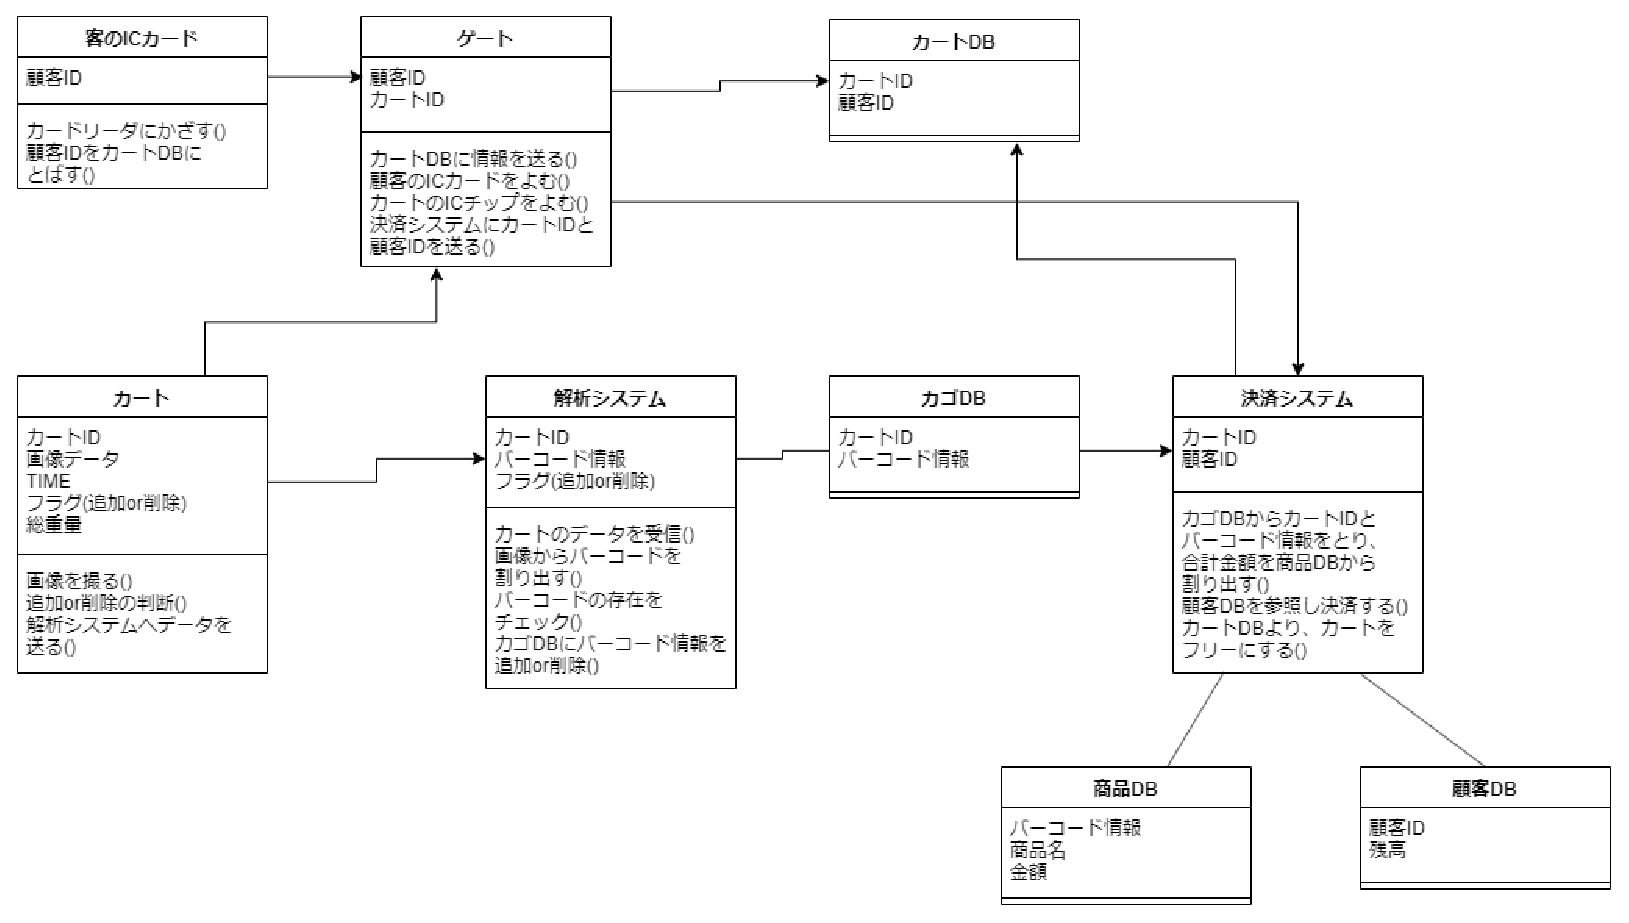
\includegraphics[width=15cm]{./picture/class_ic.eps}
\caption{ICタグを用いたシステムのクラス図}
\label{class_ic}
\end{figure}


以下にQRコードを用いた商品識別システムのクラス図,図\ref{class_qr}を載せる.


\begin{figure}[htbp]
\centering
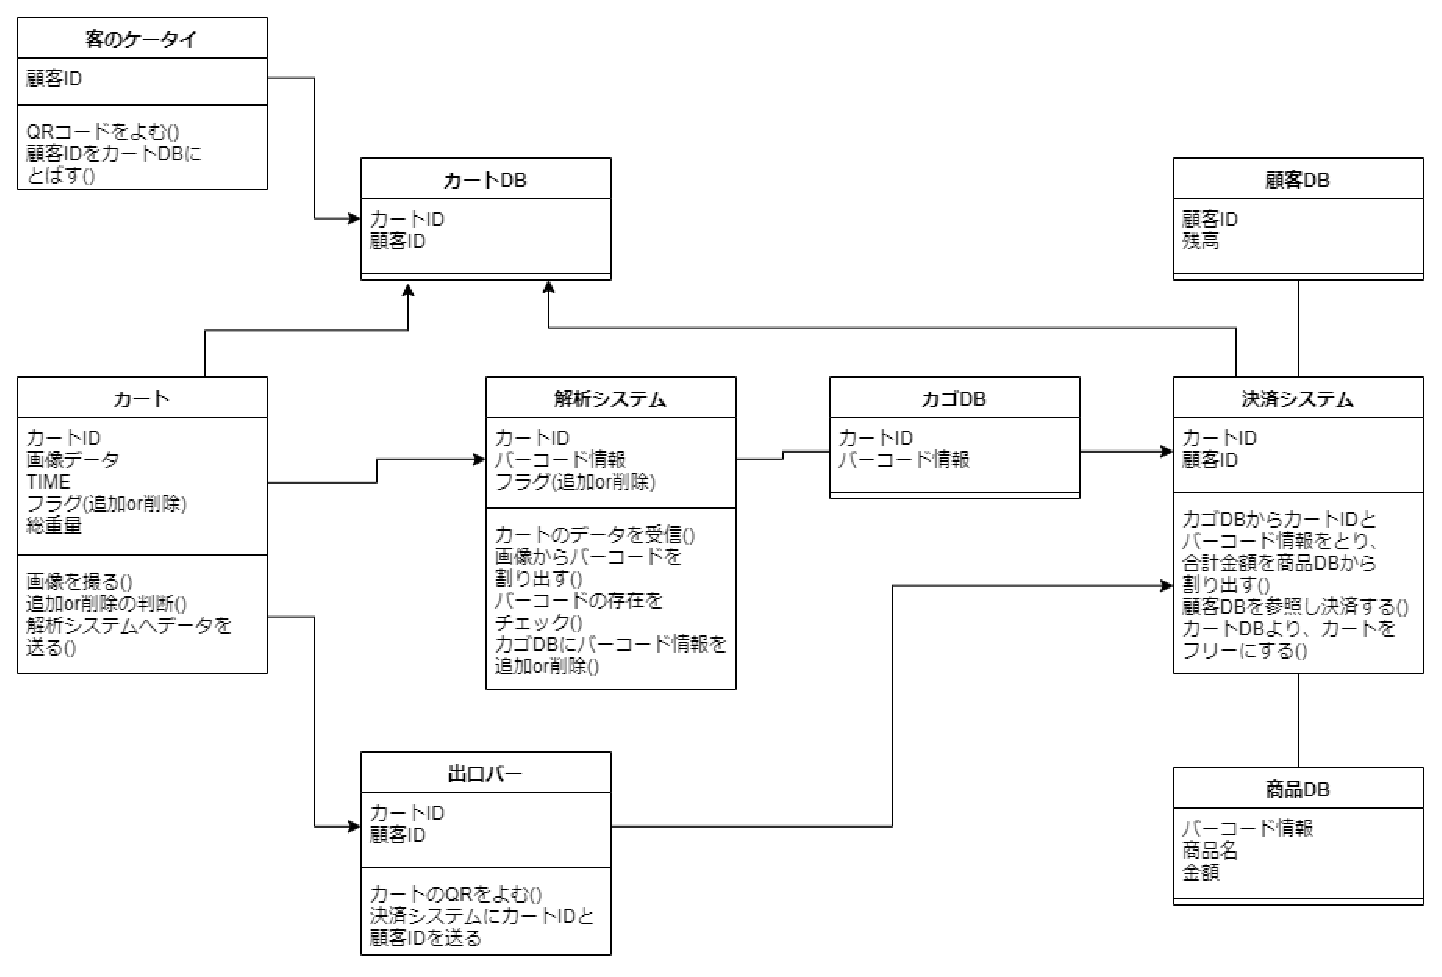
\includegraphics[height = 9cm,width=15cm]{./picture/class_qr.eps}
\caption{QRコードを用いたシステムのクラス図}
\label{class_qr}
\end{figure}


図\ref{class_ic}と図\ref{class_qr}の違いは,ユーザ情報の登録をユーザのICタグから行うか,ユーザの形態から行うかという違いである.本研究では,クラスとしてカート(カゴ)・解析システム・カゴDB・商品DBの部分を開発対象とした.開発対象となる部分については,ICタグを用いた場合とQRコードを用いた場合とで違いはないため,そのまま本研究で実装する優先度の高いシステムのクラス図をまとめて,図\ref{class_qr_2}に示す.


\begin{figure}[htbp]
\centering
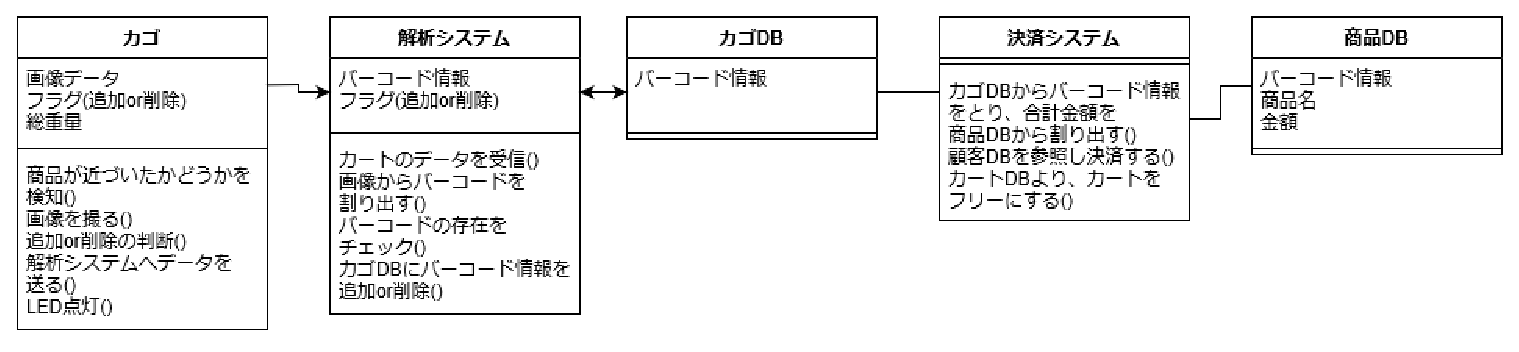
\includegraphics[width=15cm]{./picture/class_final.eps}
\caption{高優先度のシステムのクラス図}
\label{class_qr_2}
\end{figure}


図\ref{class_qr_2}において,筆者の担当した範囲はクラスとしては「カート(カゴ)」の部分である.カゴでは各種センサの制御と,解析システムへの情報の送信を行う.カゴは画像データと追加か削除のフラグ,総重量,超音波センサの情報を保持し,解析システムへ画像データとフラグをセットにし,送信する.

基本設計の段階で,それぞれの用途のために各種センサを選定した.下記に選定したセンサと選定理由を述べる.


\subsection{Webカメラの選定}


まず,バーコードを読み取る装置の選定である.本章の最初に述べた基本の評価軸より,コストを抑えられるか,従来のセミセルフレジより簡単な動作で決済まで行えるか,かつバーコードを読み取ることができる装置,加えて拡張性のある装置かどうかを基準として選定した.コストを抑えているかつバーコードを読み取ることができる装置として,バーコードリーダー,Webカメラが挙げられる.バーコードリーダーとWebカメラを比較した表を下記表\ref{came}に示す.


\begin{table}[htb]
\begin{center}
\caption{バーコードリーダーとWebカメラの比較}
\begin{tabular}{|l|c|c|} \hline
 & バーコードリーダー & Webカメラ \\ \hline \hline
価格 & 〇 2,000円台 & 〇 2,000円台 \\
動作の容易さ & ×店員と同じ動作 & △ バーコード向き制限有 \\
バーコードの読み取り可否 & 〇 & 〇 \\
拡張性 & × バーコード読み取りのみ & 〇 \\ \hline
\end{tabular}
\label{came}
\end{center}
\end{table}


価格はどちらも2,000円台から購入できるため,2,000円のバーコードリーダやWebカメラをカゴ1個につき1台分購入したとしてもカゴ90個で約180,000円とコストを抑えることが可能である.しかしながら簡単さにおいては,バーコードリーダーを使用する場合は従来のセルフレジと同じ動きをしなければならないため,×の評価がつく.Webカメラにおいては,カゴ1個につき1台を導入したとすると定点カメラとなるため,カメラ側にバーコードを向けるという手間がかかる.拡張性についてはWebカメラの場合,バーコードをカメラに向けなくても商品の形状から商品もしくは商品の種類をを特定できるようになる等の例が挙げられた.上記より要件を満たすとして,本研究ではバーコードを読み取る装置としてWebカメラを選定した.


\subsection{超音波センサの選定}


次に,ユーザが商品をカゴに出し入れした際の動作の検知を行う装置の選定を行った.消費電力を低く抑えるため,手もしくは商品が手もしくは商品がセンサの前を通った際のみにWebカメラが画像を撮影するという状況を想定した.検知するセンサとして,焦電型赤外線センサ,レーザ距離センサ,超音波センサが挙げられた.カゴの上部にセンサを設置するとしたとき,買い物カゴの奥行はおよそ360mm程であるため,その程度の距離に適しているか,また手や商品が通った時のみにセンサが反応するかを基準としてセンサの選定を行った.比較した表を下記の表\ref{kyori}に示す.


\begin{table}[htb]
\begin{center}
\caption{動作を検知するセンサの比較}
\begin{tabular}{|l|c|c|c|c|} \hline
 & 焦電型赤外線センサ & レーザ距離センサ & 超音波センサ \\ \hline \hline
価格 & 〇 500円程度 & △ 1,000円程度 & 〇 500円程度 \\
適性距離 & × 3~5m & 〇3~200cm & 〇 2~400cm \\ 
反応要件 & × 感知距離が広すぎる & △ 色による影響有 & 〇 色,形状,汚れに強い \\ \hline
\end{tabular}
\label{kyori}
\end{center}
\end{table}

上記の\ref{kyori}より,超音波センサが要件を満たしている.以上より,本研究ではユーザが商品をカゴに出し入れした際の動作の検知を行う装置として超音波センサを用いた.


\subsection{ロードセルの選定}

ユーザが商品を追加するか削除するかを判別するために,ユーザがボタンを押すなどの特別な動作をしないと考えた際,カゴの底に台を設置し,重量を検知,重量が増加すれば追加,重量が減少すれば削除と判断するとした.その際,商品の重量を検知するセンサの選定を行った.重量を検知するセンサとして,感圧センサとロードセルが候補として挙がった.基本の評価軸から,コストは抑えられるか,商品の総重量が約2kg程だとすると2kgまで検知できるかどうか,g単位で重量の増加,減少を検知できるか,カゴの底面積の半分ほどの広さとして約$255\times180mm$を最低でも検知できるかを基準とし,選定をした.比較した内容を下記の表\ref{rodo}に示す.


\begin{table}[htb]
\begin{center}
\caption{重量を検知するセンサの比較}
\begin{tabular}{|l|c|c|} \hline
 & 感圧センサ & ロードセル \\ \hline \hline
価格 & △ 1,300円程度 & 〇 600円程度 \\
検知できる重量 & 〇 100g~2kg程度  & 〇 3kg程度 \\ 
感度,精度 & △ 100g単位での検知 & 〇 g単位で検知可能 \\
検知範囲 & × 感知範囲が狭すぎる & 〇 ただし,板設置要 \\ \hline
\end{tabular}
\label{rodo}
\end{center}
\end{table}


表\ref{rodo}において,検知範囲が大きな感圧センサを比較対象として選んだものの,$40mm\times40mm$程度とカゴの約半分の底面積を検知できかねる次第であった.また,表には記載していないが,感圧センサにおいては定常的な負荷に対して徐々に抵抗値が小さくなるという特性があるため,本システムのような定常的な計測には向いていないと判断した.ロードセルにおいては,感圧センサと比較した場合広範囲の検知が可能である.以上より,重量を検知するセンサとしてロードセルを採用した.ロードセルにはひずみゲージが配置してあり,そのひずみにより重量を感知するという性質上,ひずませるための空間を作る必要があるため,ロードセルの上下に板を設置する必要がある.実装の際には,アクリル板を使用し組み立てを行った.